\section*{Scheme}
\underline{A}usdr\"ucke , \underline{A}uswertung und \underline{A}bstraktion\\
\subsection*{Dr Racket}
\fbox{
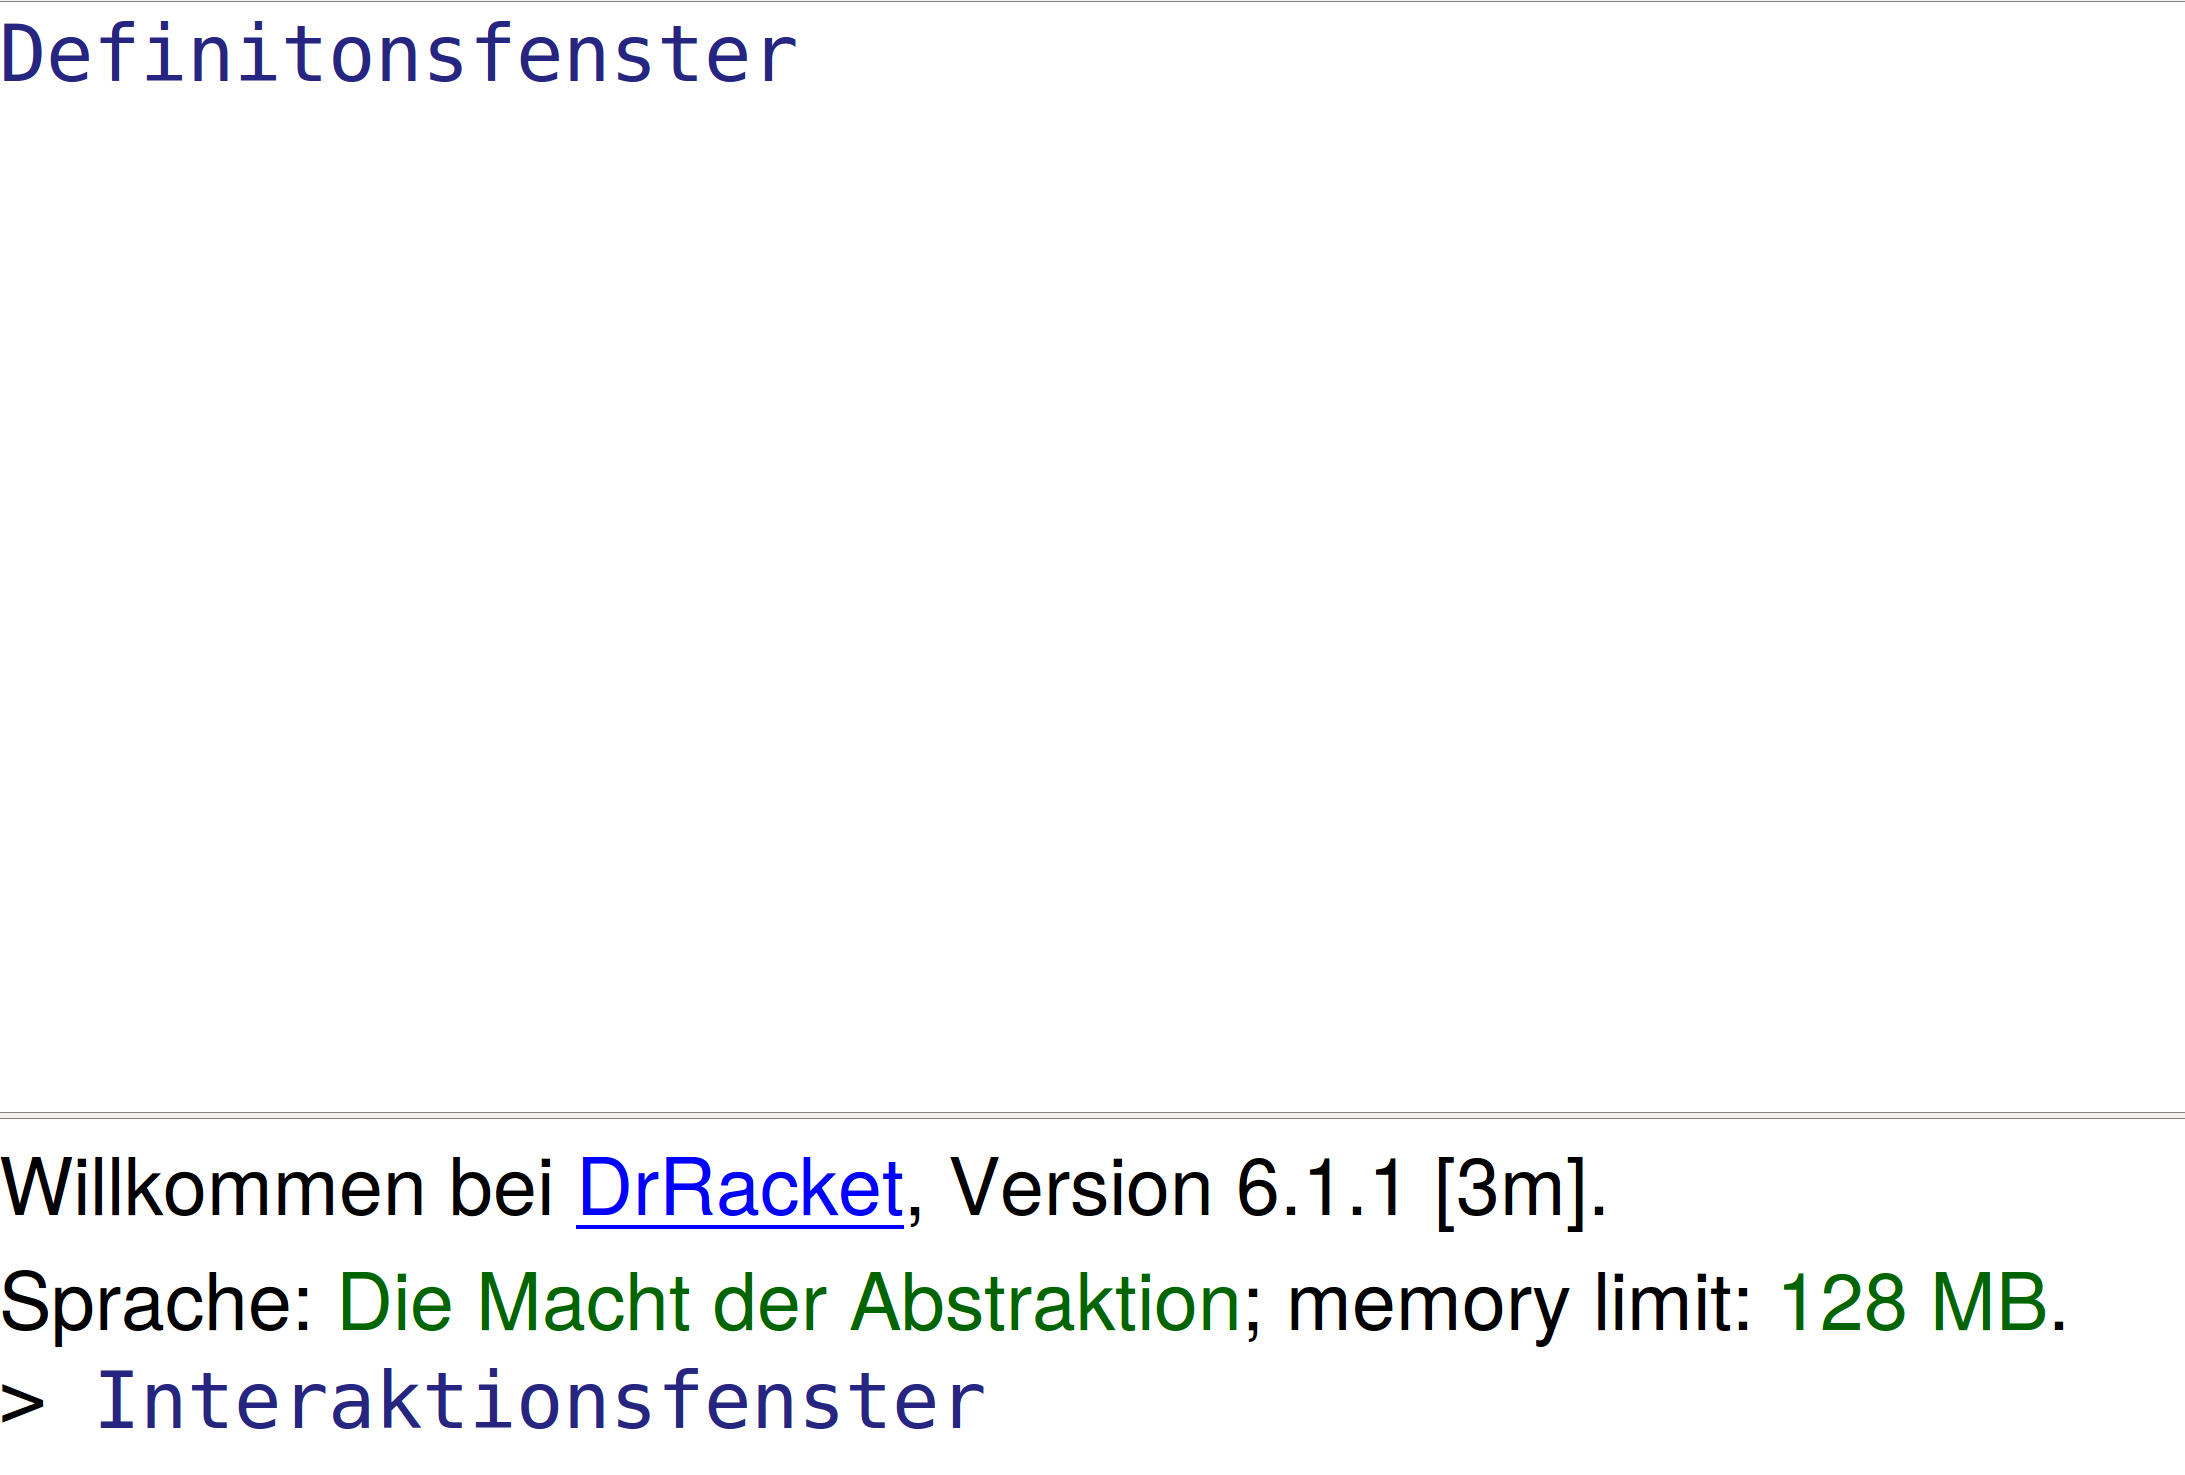
\includegraphics[scale=0.15]{drracket}}\\
Die Anwendung von Funktionen wird in Scheme ausschlie\ss lich in Pr\"afixnotation durchgef\"uhrt\\
\linie\\
\begin{center}
\begin{tabular}{c|c}
Mathematik & Scheme \\
\hline
$44-2$ & $(- $44 2)\\
$f(x,y)$ & (f x y)\\
$\sqrt{81}$ & (sqrt 81)\\
$9^2$ & (expt 92)\\
$3!$ & (! 3)\\
\end{tabular}\\
Allgemein: (\textless funktion\textgreater \textless argument1\textgreater \textless argument2\textgreater \ldots)
\end{center}
(+ 40 2) und (odd? 42) sind Beispiele f\"ur \underline{Ausdr\"ucke}, die bei \underline{Auswertung} einen Wert liefern\\
(Notation: \eval)\\
(+ 40 2) $\underbrace{\longrightsquigarrow}_{Reduktion}$ 42\\
(odd? 42) \eval \#f\\
\linie\\
Interaktionsfenster:\hspace*{2.5cm} $\underbrace{Read \rightarrow Eval \rightarrow Print \rightarrow Loop}_{REPL}$\\
\linie\\
\underline{Literale} sethen f\"ur einen konstanten Wert (auch: \underline{Konstante}) und sind nicht weiter reduzierbar.\\
\begin{center}
\begin{tabular}{ccc}
Literal &  & Sorte,Typ\\
\hline
\#f ,\#t & (true,false,Wahrheitswert) & boolean\\
"x" & (Zeichenketten) & String\\
0 1904 42 $-2$ & (ganze Zahl) & Integer\\
0.42 3.14159 & (Flie\ss kommazahl) & real\\
1\textbackslash 2, 3\textbackslash 4, -1\textbackslash 10 & (rationale Zahlen) & rational\\

\includegraphics[scale=0.2]{Darth_Vader} & (Bilder) & image

\end{tabular}
\end{center}


